%  this is a description of a cvd process usually used in this worl
There are two major ways to grow adlayers defined by their atomic constituents and certain stoichiometry in UHV, namely the chemical vapor deposition (CVD) or temperature programmed growth (TPG) of a precourser.

While the latter works by adsorption of the precourser onto the surface where it schould grow and activating the reaction via heating, the first uses a already hot surface to decompose the precourser on. 

\paragraph{CVD}\index{CVD}offers some advantages over TPG when it comes to homogenous growth of a monolayer. The precourses decomposes on contact with the hot substrate surface and its fragments for the adlayer. As time goes by, the adlayer grows in coverage and less free hot surface area is available for decomposing new ``building blocks'' for monolayer formation. If a monolayer is formed, no additional second layer is formed because of missing building blocks which only arise on contact with the uncovered substrate surface. Therefore this process is called self-limited.

While in CVD, the process of forming the adlayer (adsorption, decomposing, diffusion on surface upon coalescence with an already present nucleation seed, layer growth), TPG offers some other path of layer growth. Due to the fact that the surface is covered from the beginning with the desired number of molecules, the density of present building blocks at a certain time (and same dosage as with CVD) is higher. Therefore this growth experiences other results as CVD.

Hexagonal boron nitride grown on noble metals shows destinct differences between these two modes. CVD results in a more homogenous monolayer coverage than TPG and is therefore preferred.

The growth by itself is well investigated on transition metal surfaces \cite{gomez_diaz_hexagonal_2013,morscher_formation_2006}, on the copper and nickel surfaces \cite{preobrajenski_monolayer_2005,joshi_boron_2012}. Even more complicated samples can be created with this technique \cite{roth_chemical_2013} and the following gives a short introduction in the occuring processes.

\begin{wrapfigure}{l}{0.3\textwidth}
 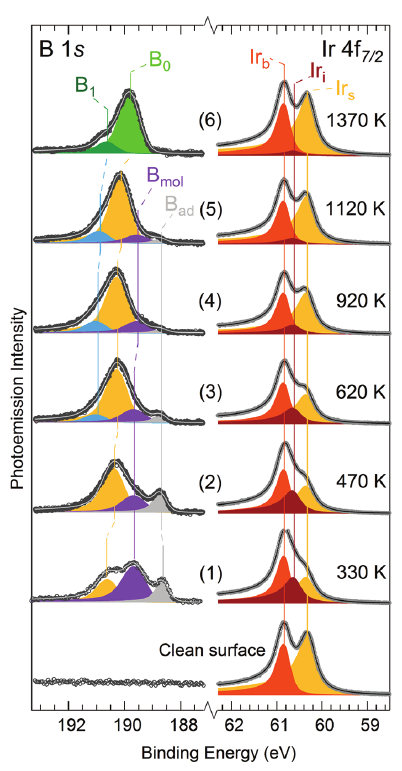
\includegraphics[width=0.9\linewidth]{./images/07571n_fig5.png}
 \caption{\cite{orlando_epitaxial_2012}}
\label{fig:borazine-TPG-on-Ir}
\end{wrapfigure}

Figure \ref{fig:borazine-TPG-on-Ir} shows a typical XPS spectrum of a TPG process with borazine adsorbed on a Iridium surface. At the graphics' bottom one can see the clean Ir surface with no borazine adsorbed (no sign of B1s). There are two contributions in the Ir-peak. While the low energy ($Ir_s$) peak stems from the surface atoms of the subtrate, $Ir_b$ denotes the contribution from the atoms in the bulk. Upon borazine adsorption $(1)$ a broad $B1s$ emerges accompanied with a new contribution in the $Ir$-peak which is a result of borazine-Ir interaction decreasing the intensity of $I_b$ and $I_s$ .

Upon annealing ($(2)$-$(6)$) this peak looses in intensity while the $I_b$ and $I_s$ recover to their initial position. Interesting changes happen to the $B1s$ peak. While at lower temperatures, several peak contributions can be distinguished, denoted as $B_{mol}$ for entire molecules and $B_{ad}$ for molecular fragments. With increasing temperature, $B_{mol}$ decreases for a increase in the $B_0$ peaks. At lower temperature (1), $B_{mol}$ decreases and $B_{ad}$ slightly increases. When exceeding 620K ($\approx \SI{350}{\celsius}$, (3)) a new peak emerges and develops into $B_1$ when increasing temperatures. When temperature is high enough the only peaks left are $B_0$ and $B_1$ - the two contributions of boron atoms stem from boron atoms interact with the Iridium substrate with different strength due to different registry to the substrate.

While usaually borazine is used as precourser different other options exist like B-Trichloroborazine (${ClBNH}_3$) \cite{auwarter_synthesis_2004-1}.